\documentclass[]{scrartcl}
\usepackage[utf8]{inputenc}
\usepackage{graphicx}
\usepackage{amsmath}
\usepackage{float}
\usepackage[ngerman, english]{babel} 
\usepackage{hyperref}
\hypersetup{
	colorlinks,
	citecolor=black,
	filecolor=black,
	linkcolor=black,
	urlcolor=black,
}
\selectlanguage{ngerman}

\title{Modellierung dynamischer Systeme  \\ Abgabe der Praktikumsaufgabe 2}

\author{Maria Lüdemann und Birger Kamp}

\begin{document}

\maketitle
\selectlanguage{ngerman}
\tableofcontents
\newpage


\section{Teilaufgabe 1 - Erdumkreisung, Fluchtgeschwindigkeit und geostationäre Bahn}
In dieser Aufgabe ist es das Ziel den Flug eines Satelliten zu modellieren die von einer Trägerrakete in eine Startposition $x0$ gebracht wird. Von dort soll der Satellit antriebslos mit einer Geschwindigkeit von $v0$ und einem Flugwinkel $\Theta$ weiterfliegen und die Erde umrunden. Ab der antriebslosen Phase $x0$ startet unsere Simulation. Dabei haben wir wie vorgegeben den Einfluss des Satelliten auf die Erde vernachlässigt und die Simulation mithilfe des gegeben MatLab-Skripts $Erdbahn.m$ visualisiert. Die gegeben Werte werden in Abb \ref{fig:1_BezeichnerDiagramm} veranschaulicht. Für die Simulation wurde aus den gegeben Werten und angeforderten Funktionen ein Simulink Schaltbild entworfen das die Simulation durchführt.

\begin{figure}[H]
\centering
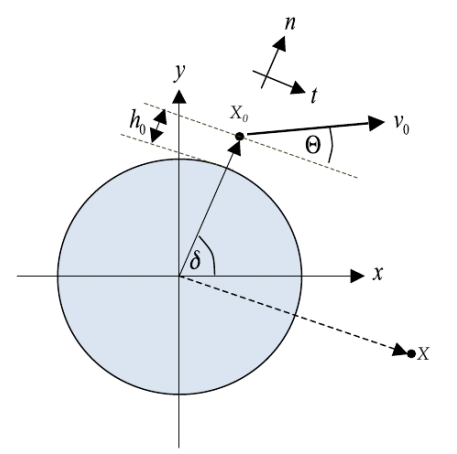
\includegraphics[width=0.5\linewidth]{./1_BezeichnerDiagramm}
\caption{}
\label{fig:1_BezeichnerDiagramm}
\end{figure}

\subsection{Gegebene Formeln und Konstanten}
Kraft auf den Satelliten
\begin{align}
\vec{F}_{S} = G \cdot \dfrac{m_{E} \cdot m_{S}}{r^2} \cdot \vec{e}_{SE}
\end{align}

Erdradius
\begin{align}
r_{E} = 6378 km
\end{align}

Erdmasse
\begin{align}
m_{E} = 5,9736 \cdot 10^{24} kg
\end{align}

Gravitationskonstante
\begin{align}
G = 66,743 \cdot 10^{-12} m^{3} kg^{-1} s^{-2}
\end{align}

\subsection{Konfigurierbare Parameter}
Folgende Parameter müssen mindestens bei der Simulation konfigurierbar sein:
\begin{itemize}
\item $v_{0}$ Startgeschwindigkeit $[km/s]$
\item $\Theta$ Flugwinkel $[^\circ]$
\item $\delta$ Startwinkel $[^\circ]$
\item $h_{0}$ Starthöhe $[km]$
\end{itemize}

\subsection{Funktionen}
Im Folgenden werden die benötigten Funktionen erklärt.

\subsection{Startposition}
Die Funktion Startposition berechnet den Startpositionsvektor $x0$ aus den gegeben Parametern $\gamma (^\circ)$ ,der Starthöhe $h0$ (km) und der Konstante Erdradius.

Dafür verwenden wir eine Formel die sich aus der Geometrie ableitet da hier mithilfe der Winkel die Ankathete und Gegenkathete der Hypotenuse von $r + h0$ berechnet werden aus denen sich die Position ableiten lässt.

Die Formel dazu beschreibt sich als 
\begin{align}
\vec{x} = [cos(\delta) \cdot( r + h0), sin(\delta) \cdot (r + h0)]
\end{align}

\subsubsection{vStart}
Die Funktion $vStart$ berechnet den Startgeschwindigkeitsvektor $\vec{v0}$ aus dem Startpositionsvektor $v0$, dem Flugwinkel $/Theta$ und dem durch die Funktion $Startposition$ berechneten Startpositionsvektor $x0$.

Um den Vektor bestimmen zu können werden zuerst die Einheitsvektoren in Tangential- und Normalrichtung ($\vec{t}, \vec{n}$ aus $x0$ konstruiert. Danach werden die Tangential- und Normalkomponenten der Startgeschwindigkeit ($v_t , v_n$) berechnet. Aus diesen Parametern lässt sich dann die Startgeschwindigkeit zusammenbauen.

Die genaue Durchfürhung findet sich im MatLab Code

\subsubsection{Beschleunigung}
Diese Funktion berechnet aus der Satellitenposition $\vec{x}$ die Satellitenbeschleunigung.
Die Kräfte die auf den Satelliten wirken summieren sich. 
\begin{align}
\Sigma{F} = m \cdot a
\end{align}
Daraus ergibt sich 

\begin{align}
a = \dfrac{\Sigma{F}}{m}
\end{align}

Wobei hier $m$ die Masse des Satelliten ist und sich heraus kürzt. Daraus folgt:

\begin{align}
a = \Sigma{F}_{SE}
\end{align}



\subsubsection{Kontakt}


\section{Teilaufgabe 2 - Mondumkreisung}

\section{Teilaufgabe 3 - Crazy Pendulum}
In dieser Teilaufgabe gilt es, die Bewegung einer Pendelkonstruktion zu berechnen. Der Versuchsaufbau ist in Abb. \ref{fig:3_Versuchsaufbau} zu sehen. In diesem Aufbau übt immer nur eine der Federn Zugkraft auf die Seiltrommel aus, während die andere Feder keine Kraft ausübt. Befindet sich das Pendel in senkrechter Position, dann übt keine der Federn eine Kraft aus. Der Einfluss der Pendelstange und der Seiltrommel werden nicht beachtet.

\begin{figure}[H]
\centering
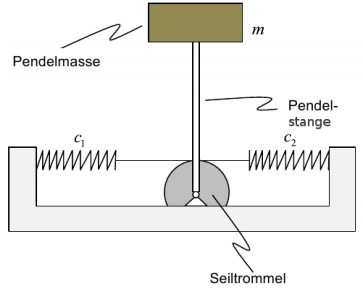
\includegraphics[width=0.5\linewidth]{./3_Versuchsaufbau}
\caption{}
\label{fig:3_Versuchsaufbau}
\end{figure}

\subsection{Formeln}
$c$ ist abhängig von $\varphi(t)$: es gilt entweder $c_{1}$ oder $c_{2}$.
\begin{align}
M_{p} = m \cdot g \cdot sin(\varphi) \cdot (L + \dfrac{h}{2})\\
M_{s} = -\varphi \cdot c \cdot r^2\\
M_{g} = M_{p} + M_{s}\\
J_{p} = \dfrac{1}{12} \cdot m \cdot (h^2 + w^2)\\
J_{g} = J_{p} + m \cdot (L + \dfrac{h}{2})^2\\
a = M_{g}/J_{g}
\end{align}
$a$ wird in der Einheit $Grad/s^2$ angegeben.

\subsection{Simulink-Modell}
Die Berechnung von $a$ erfolgt in der Embedded-MatLab-Function \textit{fcn}.

\begin{figure}[H]
\centering
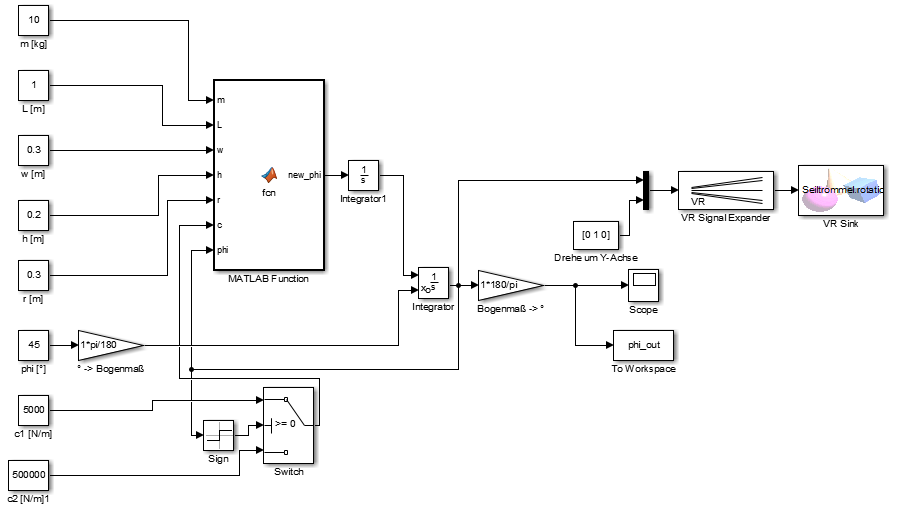
\includegraphics[width=1\linewidth]{./3_Modell}
\caption{}
\label{fig:3_Modell}
\end{figure}

\subsection{Plot des Ergebnis}
Die Abbildung \ref{fig:3_Plot} zeigt $\varphi(t)$ des Modells als Plot. Die Abstände und Maximalstellen der Kurve verändern sich während der Laufzeit nicht nennenswert. Sie bleiben nahezu gleich, eine Veränderung ist nur an der dritten Nachkommastelle zu sehen.

\begin{figure}[H]
\centering
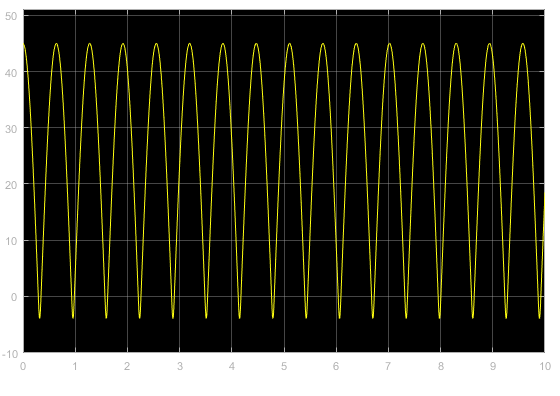
\includegraphics[width=0.5\linewidth]{./3_Plot}
\caption{}
\label{fig:3_Plot}
\end{figure}

\section{Teilaufgabe 4 - Schwingungsgedämpfter Tisch}


\end{document}
